\section*{Análise dos Gráficos com Vento em Z}

\subsection*{Gráfico da Guinada (Yaw)}
Observando o gráfico da guinada sob a influência do vento em Z (Figura \ref{fig:windz-yaw}), percebe-se que a guinada verdadeira sofre uma oscilação significativa, especialmente nos primeiros segundos, com amplitude máxima ao redor de \(6 \times 10^{-4}\) radianos. O sinal estimado consegue acompanhar essas variações iniciais com menor amplitude, mostrando um efeito de amortecimento em relação à guinada verdadeira. A guinada de referência permanece constante em zero, indicando que o sistema está tentando manter a orientação original, mas é perturbado pela influência do vento.

\begin{figure}[h!]
    \centering
    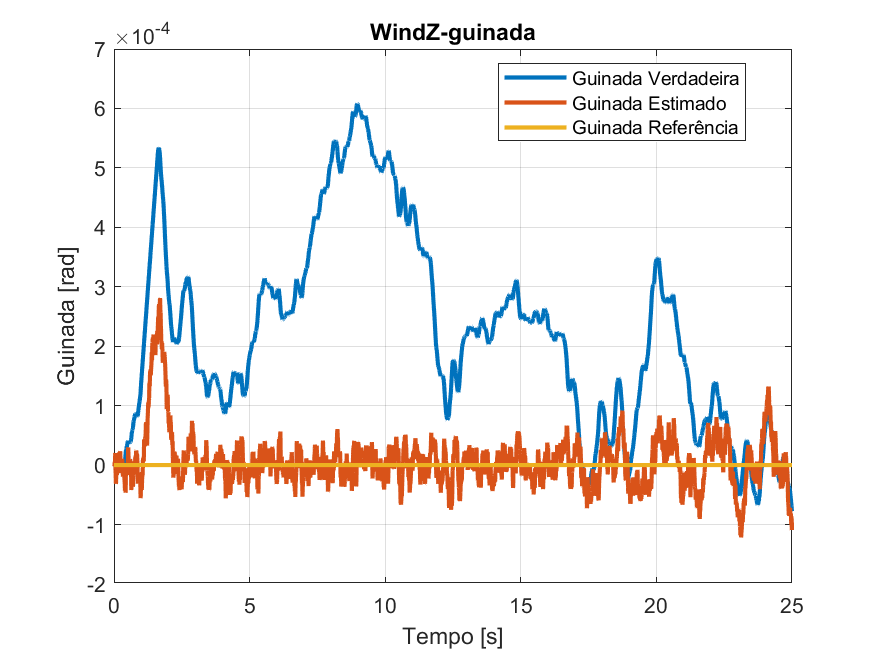
\includegraphics[width=0.8\textwidth]{WindZ-guinada.png}
    \caption{Gráfico da guinada com vento em Z.}
    \label{fig:windz-yaw}
\end{figure}

\subsection*{Gráfico da Arfagem (Pitch)}
O gráfico da arfagem (Figura \ref{fig:windz-pitch}) mostra uma resposta oscilatória inicial com diminuição gradual da amplitude ao longo do tempo. O sistema de controle se esforça para manter a arfagem próxima à referência, que é zero, mas a presença do vento causa pequenas oscilações que se estabilizam lentamente. O sinal estimado e o comando estão próximos ao sinal verdadeiro, sugerindo que o controlador consegue amortecer essas oscilações, mas com dificuldade de alcançar uma estabilidade imediata.

\begin{figure}[h!]
    \centering
    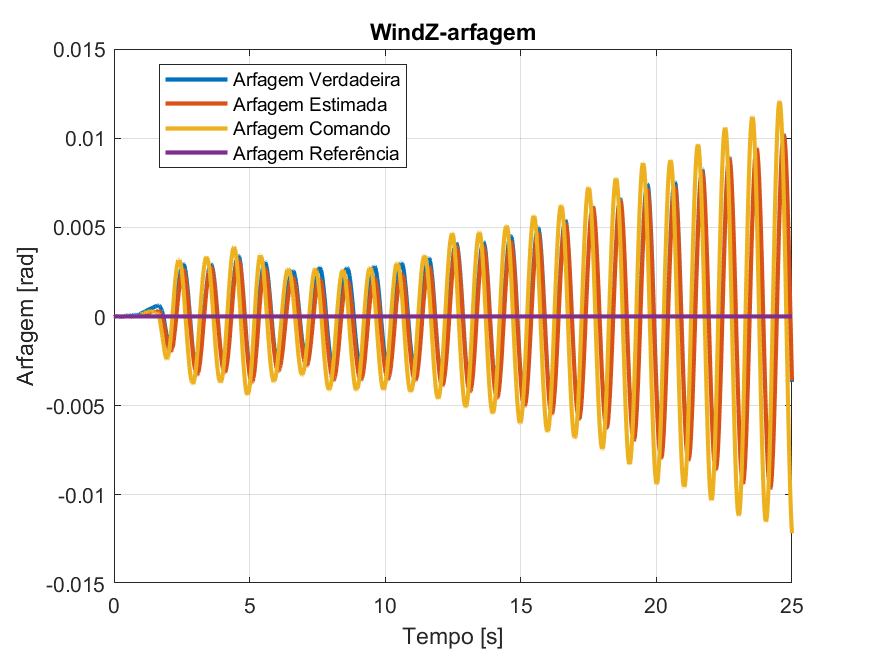
\includegraphics[width=0.8\textwidth]{WindZ-arfagem.png}
    \caption{Gráfico da arfagem com vento em Z.}
    \label{fig:windz-pitch}
\end{figure}

\subsection*{Gráfico da Rolagem (Roll)}
No gráfico de rolagem (Figura \ref{fig:windz-roll}), também observamos oscilações significativas causadas pelo vento, com uma amplitude menor do que a da guinada e da arfagem. A rolagem verdadeira é acompanhada de perto pela estimativa e pelo comando, com uma resposta bem próxima ao sinal de referência ao longo do tempo. O controlador consegue mitigar bem os efeitos do vento em Z na rolagem, indicando uma estabilidade razoável nesse eixo.

\begin{figure}[h!]
    \centering
    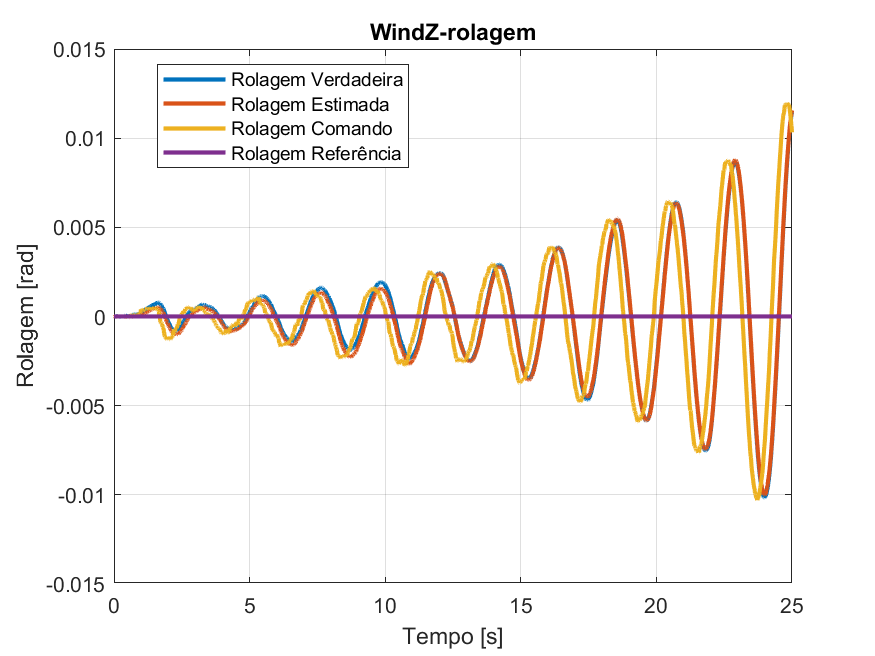
\includegraphics[width=0.8\textwidth]{WindZ-rolagem.png}
    \caption{Gráfico da rolagem com vento em Z.}
    \label{fig:windz-roll}
\end{figure}

\subsection*{Gráfico da Coordenada Z}
No gráfico da coordenada Z (Figura \ref{fig:windz-z}), o impacto do vento é observado como uma queda inicial na altura do drone, que se recupera e estabiliza próximo ao valor de referência, que está em -2 metros. A estimativa acompanha essa queda e recuperação, mostrando que o controlador consegue restaurar a altura desejada após as perturbações iniciais, mantendo o drone estável na altitude pretendida.

\begin{figure}[h!]
    \centering
    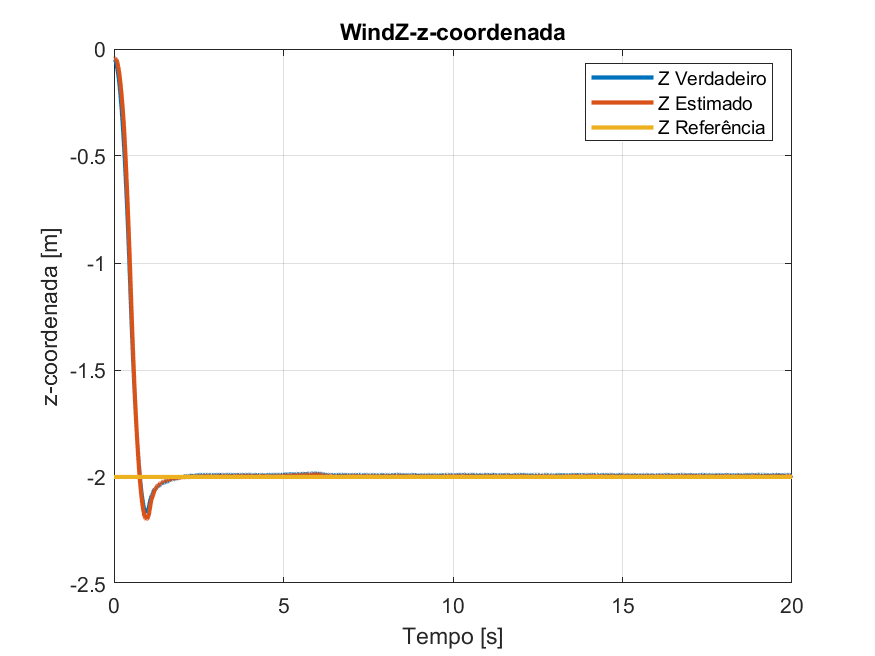
\includegraphics[width=0.8\textwidth]{WindZ-z-coordenada.png}
    \caption{Gráfico da coordenada Z com vento em Z.}
    \label{fig:windz-z}
\end{figure}

\subsection*{Gráfico da Coordenada Y}
A coordenada Y (Figura \ref{fig:windz-y}) mostra uma oscilação ao longo do tempo, com uma resposta do sistema que leva o drone a flutuar em torno do ponto de referência, que é zero. O sinal estimado é muito próximo do verdadeiro, porém levemente desfasado, o que pode ser um efeito residual da influência do vento em Z, levando o sistema a uma oscilação residual que persiste ao longo do tempo.

\begin{figure}[h!]
    \centering
    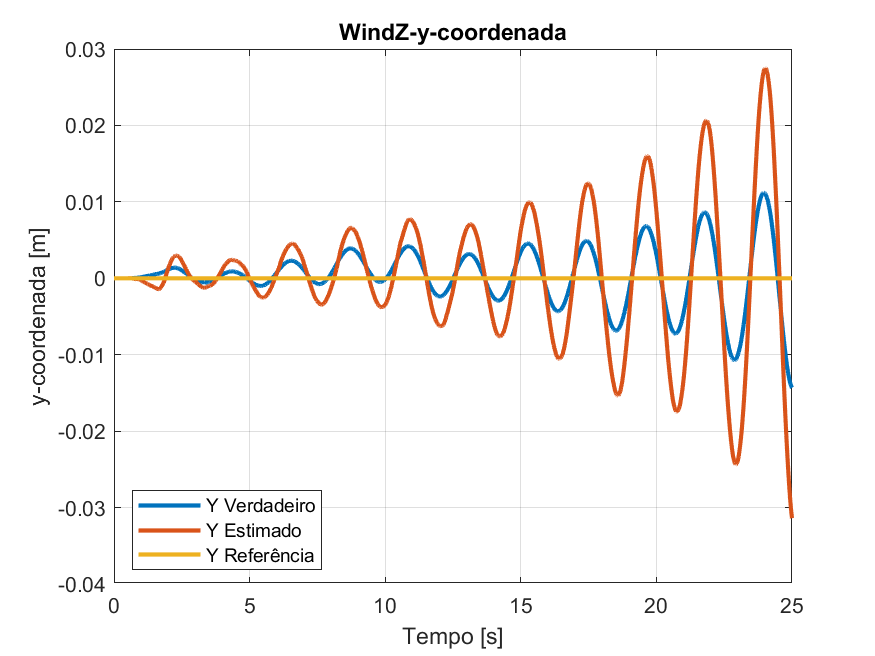
\includegraphics[width=0.8\textwidth]{WindZ-y-coordenada.png}
    \caption{Gráfico da coordenada Y com vento em Z.}
    \label{fig:windz-y}
\end{figure}

\subsection*{Gráfico da Coordenada X}
Por fim, na coordenada X (Figura~\ref{fig:windz-x}), o comportamento é similar ao da coordenada Y, com oscilações de pequena amplitude que são amplificadas pelo vento, especialmente após os primeiros segundos. O sinal estimado e o verdadeiro se mantêm próximos, mas a perturbação causada pelo vento impede uma convergência exata à referência, resultando em um erro residual pequeno e oscilatório.

\begin{figure}[h!]
    \centering
    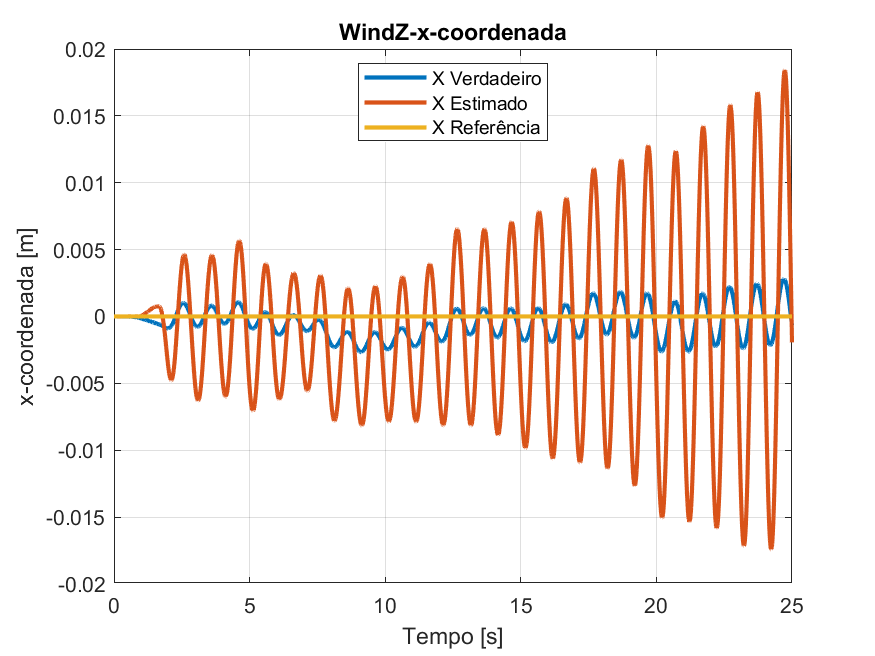
\includegraphics[width=0.8\textwidth]{WindZ-x-coordenada.png}
    \caption{Gráfico da coordenada X com vento em Z.}
    \label{fig:windz-x}
\end{figure}

%\section*{Conclusão}
%A análise dos gráficos sob a influência de vento no eixo Z revela que o sistema consegue, em grande parte, manter a estabilidade e reduzir os efeitos das perturbações, especialmente na altitude e rolagem. No entanto, a guinada e a arfagem apresentam respostas mais sensíveis, com oscilações amortecidas ao longo do tempo. Em resumo, o controlador consegue minimizar os impactos do vento, mas algumas oscilações residuais permanecem nos eixos horizontal e de orientação.

%---------------------------------------------------------------------
% INDICE REMISSIVO
%---------------------------------------------------------------------
\phantompart
\printindex
%---------------------------------------------------------------------
